

\begin{figure}
\vspace{-4mm}
    \centering
    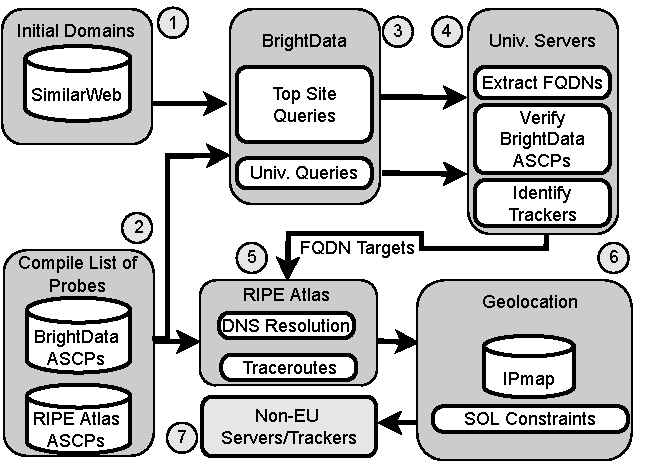
\includegraphics[width=.46\textwidth]{figures/DataLoc-Methodology-v2.pdf}\\
    \caption{Process diagram summarizing our methodology. Steps numbered (1)\&(2) are data sources. 
Steps (3)\&(4) are browser-based measurements. Steps (5)\&(6) are data-plane measurements. 
Step (7) refers to rDNS filtering and the final output. All steps are referenced in our method sections.}
\label{fig:methodoverview}
\vspace{-4mm}
\end{figure}

\section{Network \& Country Sample}
Our method ensures that we launch both browser-based and network measurements
from the same network and in the same country. (We do not collect any personal 
information; we include an ethics section in the appendix). This constraint significantly increases the likelihood 
that both the DNS resolution, and therefore also the responding server, are 
identical in both sets of measurements. To this end, we identify overlaps in the
measurement infrastructure provided by two platforms: RIPE, the European Internet registrar
that hosts RIPE Atlas~\cite{atlas}, a large-scale Internet measurement
platform with very dense deployment in the EU; and BrightData, a large-scale proxy service~\cite{BrightData}.
To compute this overlap, we look at the networks present in each EU country that are represented
in each platform. We evaluate networks at the granularity of Autonomous Systems (AS),
the administrative domain over which a company (network operator) has control over;
ASes are the entities explicitly named in entries on the routing system, the Border Gateway Protocol, that rules
over how traffic is delivered in the global Internet. 
We thus look for AS-Country Pairs (ASCPs), or an AS in a country--a single AS can operate in 
multiple countries--where both platforms host a probe, step (2) of Fig.~\ref{fig:methodoverview}.

While RIPE regularly publishes a list of its active probes~\cite{RipeAtlasInfo},
including country and AS,
BrightData does not provide a list of active networks in each country. 
To find BrightData's AS-Country Pairs in the EU, we send repeated queries to request 
a proxy in a specific country over a period of two weeks in the last quarter of 2021. 
We find that while RIPE has presence in 2,957 ASCPs,
BrightData is present in 4,037. The intersection is 1,355 ASCPs, covering 1,318 ASes in 27 countries.

\subsection{BrightData Justification}
BrightData ensures that traffic comes from 1,000+ residential EU networks, reflecting what EU residents see on their browsers. 
Other proxy services lack this coverage. 
Further, RIPE Atlas, while widespread in the EU, lacks a browser to execute JavaScript, 
limiting its capability; data center-based approaches, meanwhile, are easily detectable and treated differently by content providers. 
Although BrightData can not load Google domains as initial sites, 
we observed 25 out of 41 Google domains (see \S~\ref{sec:googledoms}) as third parties on non-Google sites, 
capturing key interactions between browsers and Google properties.
We conduct an experiment to validate BrightData's proxy locations in \S~\ref{sec:proxyval}.

\section{Identifying Relevant Domains \& Trackers}
\label{sec:domains}
In this section, we describe our identification of relevant, popular
domains in each EU country, step (1) in Fig.~\ref{fig:methodoverview}. 
Our code and data is available on GitHub.~\cite{githubrepo}

\subsection{Initial Sample of Top Sites per EU Country}
We rely on a list of the top 50 websites in each EU country published by SimilarWeb~\cite{SimilarWeb}, 
which has also been used in previous studies~\cite{bui2022opt,zheutlin2021data}. 
SimilarWeb is the source of initial domains represented in step (1) of Fig.~\ref{fig:methodoverview}.
From this list, we exclude 19 adult sites as queries to them are not permitted by BrightData. 
 SimilarWeb has no list of top sites in 7 smaller EU countries,
so we exclude them from our sample.
We are left with 604 websites in 20 countries. 

To obtain a representative sample of popular websites in each EU country, 
we used SimilarWeb instead of Tranco,~\cite{Tranco}
as tranco primarily focuses on global rankings. 
Previous work has shown
that global website lists are skewed toward certain nations and do not reflect regional experiences.~\cite{ruth2022world}
However, to determine whether Tranco would have included 
the same regionally-popular sites, and thus would have been a reasonable alternative to SimilarWeb for our purposes, we analyzed
the percentage of top 50 websites in each EU country (based on SimilarWeb) that appeared in the Tranco list. 

We find that Tranco would be an unsuitable replacement for SimilarWeb.
Across all 20 countries, collectively, only 18\% of the top 50 
SimilarWeb websites were included in Tranco top 50. 
This percentage increased to 24\% for Tranco top 100 and 32\% for its top 1,000.
Figure ~\ref{fig:tranco} illustrates this limited overlap between similarweb country specific rankings and Tranco global rankings. 
\begin{center}
\begin{figure}
    \centering
    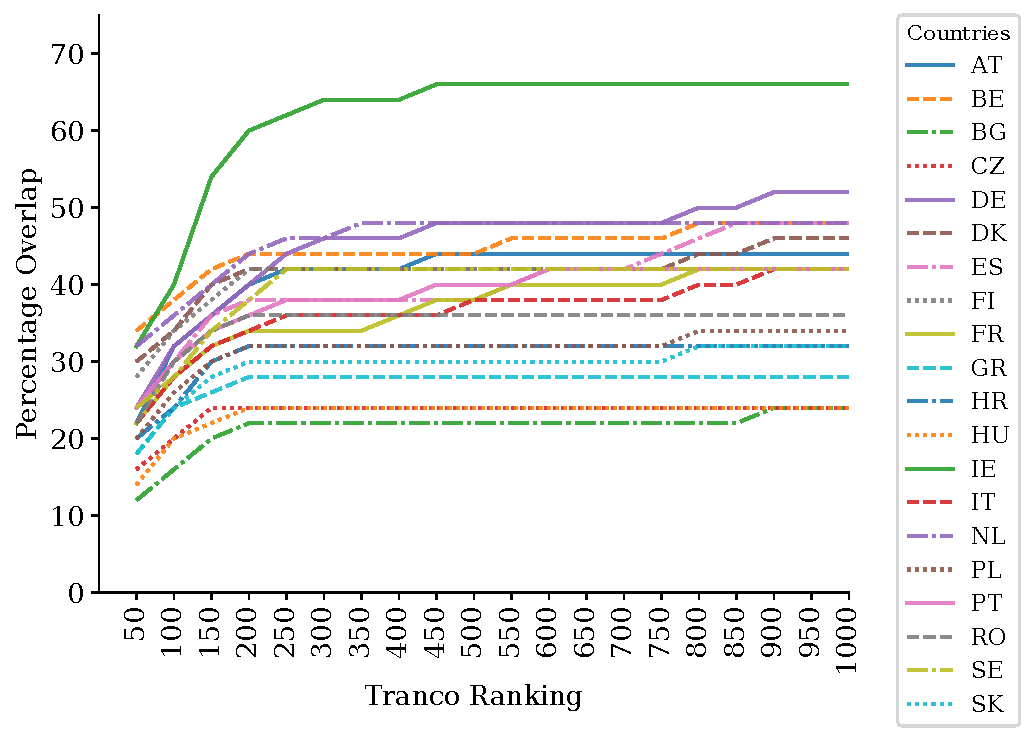
\includegraphics[width=\linewidth]{figures/tranco.pdf}\\
    \caption{Percentage of overall agreement between Tranco and SimilarWeb lists.}
\label{fig:tranco}
\vspace{-6mm}
\end{figure}
\end{center}


\subsection{Identification of First Parties}
\label{sec:firstparty}
To identify linked domains owned by the same entity
as the site that requests them, 
we follow a set of simple heuristics.
First, we look for AS number match derived from a sequence of
DNS resolution (in our local machine) and IP-to-AS lookup from Team Cymru~\cite{cymru}. If two domains resolve to an IP owned by 
the same AS, we infer that the domains belong to the same company and
thus the linked domain is a first party.
We similarly label domains as first parties if there is an 
organization match (using the AS from Team Cymru as an input)
in CAIDA's AS2Org database~\cite{astwoorg}.
Domains that are not first parties are then labeled as third parties.

We note that this method will produce a lower bound for 
third-party domains loaded by the initial target sites and
thus present in our data. Since our labeling of third-parties
is primarily used for finding known trackers that are missed by 
existing databases (\S~\ref{sec:trackerlabels}), 
we argue that ours is an acceptable method for labeling
domains as third parties for the scope of this paper.
We do not aim to identify every third party tracker, 
only to provide a reasonable (conservative) estimate of their prevalence,
particularly those hosted in non-adequate destinations,
in requests sent from the EU. 

\subsection{Treatment of Google Domains}
\label{sec:googledoms}
BrightData imposes restrictions on queries to Google-owned domains. 
(The reasons for these restrictions are part of a proprietary agreement
between the two companies.)
Should these queries be sent by the user, BrightData will automatically route them
through a ``superproxy,'' which is not in the ASCP that we intend to query,
deeming the results of these queries with little value for our exploration of 
data localization compliance. Thus, we are forced to exclude Google-owned properties
from our set of initial targets.

To identify Google-owned domains, we follow the first party
identification heuristics (\S~\ref{sec:firstparty}). 
Using these techniques, we identify 41 Google-owned sites
in the set of top sites from SimilarWeb. 
From these 41 sites, 28 match one of three patterns: `\url{google.TLD}',
`google.co.TLD' or `google.com.TLD', where TLD refers to any country's top-level domain, such as 
`.bg'. We also include youtube.com and news.google.com in this list, as they are well-known Google sites. 
All but 4 of these, or 24 domains, 
are present in at least one non-Google-owned site: on average, these sites
appear in more than 2,000 DNS requests from other sites--they are embedded in a vast 
number of non-Google-owned sites
in many EU countries. 
BrightData does 
allow these queries, where a Google site is loaded by a non-Google site, 
to be routed through the requested ASCP.

Of the 13 additional sites owned by Google in our set of top sites,
1 is loaded by a non-Google-owned domain. 
In sum, we are only unable to measure data localization compliance for 
16 Google-owned top sites, as the remainder are requested by non-Google sites. 
These represent less than 1\% of our target
sites from the previous subsection. 

We do acknowledge a limitation of our method (\S~\ref{sec:domexc} lists this paper's
limitations). By not directly loading the 41 Google-owned sites,
we may be missing additional trackers that target EU users. However, this limitation is mitagated
since the majority of these sites (26)
reference Google search's frontpage for a specific country, a relatively simple website that
does not typically embed a large number of non-Google sites. The limitation is further mitigated
by the fact that these frontpage Google sites are widely present in non-Google sites, so we 
are still able to infer their data localization compliance with our method (as noted
earlier, BrightData does
allow proxies to load Google sites if they are fetched by a different initial target domain).

\subsection{Final Sample of Top Sites}
To maximize response rates, we attempt to query multiple URLs for each top site.
Since a website might be responsive to only `http' or `https' requests~\cite{paracha2020deeper}, 
we attempt to query `https' first, and if we receive no response, 
we attempt `http'. Finally, we note that some sites only respond to queries
with `www.' as a prefix to the TLD+1 domain, for instance, `www.wikipedia.org' instead of
`wikipedia.org'. In sum, we attempt 4 queries for each top site, with each
subsequent query only run if the previous one failed:
\url{https://www.website.com}, \url{http://www.website.com}, \url{https://website.com}, \url{http://website.com}.

After executing our queries through BrightData
in each ASCP, we receive responses from 
534 popular sites in 20 EU countries. 

\subsection{Web Crawls Through BrightData}
\label{sec:crawling}
We ``browse'' all popular sites in each country and record their response,
step (3) of Fig.~\ref{fig:methodoverview}.
This data collection occurred in August of 2022.
Our aim is to avoid triggering anti-bot/anticrawl measures that (likely most) popular 
sites implement.
To reach this goal, we use a headless instance of Selenium with requests routed through a 
BrightData proxy: these proxies are set up on real users, and Selenium is 
a properly configured web browser (not a command-line tool such as curl).
In practical terms, we submit HTTP/HTTPS requests to each popular site in each country from
all ASCPs identified earlier. The request is sent to the target site through BrightData using 
a Python proxy handler that is initially set up for each ASCP 
with authentication information (our user ID and a plaintext passphrase),
and the proxy port.
A BrightData proxy handler follows this expression--in addition to the
previously identified fields, TCC is the two-letter country code of the requested proxy:
\begin{verbatim}
http://lum-auth-token-country-<TCC>:<passphrase>
\end{verbatim}
\begin{verbatim}
@pmgr-customer-<user\_ID>.zproxy.lum-superproxy.io:<port>
\end{verbatim}

The output of this stage is a set of DNS requests initiated by the browser, 
which executes JavaScript and other
dynamic content. These requests include the initial target site along with any 
additional domains loaded by it. These domains are the necessary information 
for our further analyses.
While the remainder of our experiments are 
based on these DNS requests, step (4) of Fig.~\ref{fig:methodoverview}, 
we also record the web contents and cookies.

\subsection{Labeling Trackers}
\label{sec:trackerlabels}
Tracking sites pose a special concern from a privacy perspective. Thus in our 
analysis we investigate compliance with data localization by all domains,
in general, and by tracking domains, in particular. 
This is depicted in step (4) of Fig.~\ref{fig:methodoverview}.
To label a domain as a tracking site, we use a three-step approach
applied to the domains found in the Selenium DNS requests (\S~\ref{sec:crawling}).
First, we intersect the domains with known trackers from the well-established list,
EasyList~\cite{EasyList}. After manually inspecting the 256 third party domains (\S~\ref{sec:firstparty}) 
we labeled as non-trackers
following this step, we found that the vast majority still appeared to be trackers. 
Thus, second, we complement EasyList with a well-known list of trackers
(with over 1k stars) on GitHub ~\cite{GitHosts}; this process yields
an additional 167 trackers. 
Third, 
for completeness, we manually inspect the remainder third party non-trackers. 
We find five additional trackers, four of which are labeled as so because of
information in their frontpage or `about us' section (\url{24media.gr}, \url{almatalent.fi}, 
\url{cdn-expressen.se}, \url{mailchimp.com}), and 
one from their WHOIS registration (labeled as `Tech Adverts', \url{amlimg.com}).
 
With our final list of tracking domains, we then manually verify 
their labeling as third-party trackers. This manual verification is necessary 
because many sites are incorrectly labeled as first parties with 
our automated approach because the initial domains 
are also hosted by a company that
itself operates a known tracker (and thus they are
delivered to users from the same network, \textit{e.g.},
the same autonomous system). For instance,
initial target site \textit{topky.sk} in Slovakia is
hosted by Google (server IP: 172.217.2.202), 
which also operates known tracker
\textit{ajax.googleapis.com}. Our automated method thus 
concludes that the latter is a first-party of the former,
when in reality they are likely not.

To verify third-party labels, we thus rely on a manual 
verification process that leverages three primary sources:
Google search of the sites involved and their ownership, 
\textit{WhoTracks.Me}~\cite{whotracksme}, a well-known database
of online trackers, and the Whois database of domain registration 
information~\cite{whois}. Given the time-intensive nature
of this verification, we restrict this analysis to the
known trackers inferred to be in non-adequate countries
by our server geolocation method (\S~\ref{sec:servergeolocation}).
